%%%%%%%%%%%%%%%%%%%%%%%%%%%%%%%%%%%%%%%%%%%%%%%%
% E.Pinault-Bigeard - e.pinault-bigeard@upsti.fr
% http://s2i.pinault-bigeard.com
% CC BY-NC-SA 2.0 FR - http://creativecommons.org/licenses/by-nc-sa/2.0/fr/
%%%%%%%%%%%%%%%%%%%%%%%%%%%%%%%%%%%%%%%%%%%%%%%%
\documentclass[11pt]{article}
%%%%%%%%%%%%%%%%%%%%%%%%%%%%%%%%%%%%%%%%%%%%%%%%
% Package UPSTI_Document
%%%%%%%%%%%%%%%%%%%%%%%%%%%%%%%%%%%%%%%%%%%%%%%%
\usepackage{subcaption}
\usepackage[usenames, svgnames, dvipsnames]{xcolor}
\usepackage{UPSTI_Document}
\definecolor{darkspringgreen}{rgb}{0.09, 0.45, 0.27}

%---------------------------------%
% Paramètres du package
%---------------------------------%

% Version du document (pour la compilation)
% 1: Document prof
% 2: Document élève
% 3: Document à publier
\newcommand{\UPSTIidVersionDocument}{1}

% Variante
%\newcommand{\UPSTIvariante}{2}

% Classe
% 1: PTSI				6: PSI*			11: TSI2		16: Spé
% 2: PT	(par défaut)	7: MPSI			12: ATS
% 3: PT*				8: MP			13: PC
% 4: PCSI				9: MP*			14: PC*
% 5: PSI				10: TSI1		15: Sup
%\newcommand{\UPSTIidClasse}{2}

% Affichage personnalisé de la classe
\newcommand{\UPSTIclasse}{Première STI2D}

% Matière
% 1: S2I (par défaut)    2: IPT     3: TIPE
% 6: Vie au lycée
\newcommand{\UPSTIidMatiere}{4}

% Type de document
% 0: Custom*				7: Fiche Métho de			14: Document Réponses
% 1: Cours (par défaut)		8: Fiche Synthèse    		15: Programme de colle
% 2: TD     				9: Formulaire
% 3: TP						10: Memo
% 4: Colle					11: Dossier Technique
% 5: DS						12: Dossier Ressource
% 6: DM						13: Concours Blanc
% * Si on met la valeur 0, il faut décommenter la ligne suivante:
%\newcommand{\UPSTItypeDocument}{Custom}
\newcommand{\UPSTIidTypeDocument}{1}

% Titre dans l'en-tête
\newcommand{\UPSTItitreEnTete}{Communiquer}
%\newcommand{\UPSTItitreEnTetePages}{UPSTItitreEnTetePages}
%\newcommand{\UPSTIsousTitreEnTete}{UPSTIsousTitreEnTete}

% Titre
%\newcommand{\UPSTItitrePreambule}{Qu'est-ce qu'un réseau ?}
\newcommand{\UPSTItitre}{Vous êtes-vous déjà demandé comment ça fonctionne ?}

% Durée de l'activité (pour DS, DM et TP)
\newcommand{\UPSTIduree}{1h}

% Note de bas de première page
%\newcommand{\UPSTInoteBasDePremierePage}{Note de bas de 1ère page}
% Numéro (ajoute " n°1" après DS ou DM)
%\newcommand{\UPSTInumero}{1}

% Numéro chapitre
\newcommand{\UPSTInumeroChapitre}{5}

% En-tête customisé
%\newcommand{\UPSTIenTetePrincipalCustom}{UPSTIenTetePrincipalCustom}

% Message sous le titre
%\newcommand{\UPSTImessage}{Message sous le titre}

% Référence au programme
%\newcommand{\UPSTIprogramme}{\EPBComp \EPBCompP{B1-02}, \EPBCompP{B2-49}, \EPBCompS{B2-50}, \EPBCompS{B2-51}, \EPBCompP{C1-07}, \EPBCompP{C1-08}}

% Si l'auteur n'est pas l'auteur par défaut
%\renewcommand{\UPSTIauteur}{WWOOOOOOWW}

% Si le document est réalisé au nom de l'équipe
%\newcommand{\UPSTIdocumentCollegial}{1}

% Source
%\newcommand{\UPSTIsource}{UPSTI}


% Version du document
\newcommand{\UPSTInumeroVersion}{1.0}

%-----------------------------------------------
\UPSTIcompileVars		% "Compile" les variables
%%%%%%%%%%%%%%%%%%%%%%%%%%%%%%%%%%%%%%%%%%%%%%%%


%%%%%%%%%%%%%%%%%%%%%%%%%%%%%%%%%%%%%%%%%%%%%%%%
% Début du document
%%%%%%%%%%%%%%%%%%%%%%%%%%%%%%%%%%%%%%%%%%%%%%%%
\begin{document}
\UPSTIbuildPage

\section{Pourquoi et comment communiquer ?}
De tout temps, les humains ont ressenti et ressentent le besoin de communiquer.
Les méthodes dont nous nous servons pour partager idées et informations changent et évoluent sans cesse. Si le réseau humain se limitait autrefois à des conversations en face à face, aujourd'hui les découvertes en matière de supports étendent sans cesse la portée de nos communications. De la presse écrite à la télévision, chaque innovation a développé et amélioré nos moyens de communication.

\UPSTIdefinition[C'est quoi internet ?]{
Internet est un ensemble de réseaux interconnectés à l'échelle internationale qui échangent des informations selon des normes communes en utilisant des câbles téléphoniques, des câbles à fibre optique, des transmissions sans fil et des liaisons par satellite.

\UPSTIlignesACompleter[1]{Internet n'appartient à personne}
}

% A retenir
\UPSTIdefinition[Réseau]{\UPSTIlignesACompleter{Définir un réseau, c'est définir des \textbf{liens}. Un réseau désigne un ensemble de relations.
Dans le cas d'un réseau informatique, il s'agit d'un ensemble de machines (hôtes) interconnectés.}}

\subsection{Communiquer des données}
Tous les jours, nous entendons parler de données. Méta-données, big-data, données personnelles, etc. Mais que sont ces données et comment circulent-elle dans les réseaux ?

\UPSTIdefinition[Données]{Les données sont une valeur qui représente quelque chose.
Ce sont les informations sous leur forme brute ou non organisée représentant quelque chose.
}

\begin{UPSTIactivite}
  \UPSTIquestion{Citez aux moins 5 exemples de types de données que vous utilisez tous les jours.}
  \UPSTIpointilles

  \UPSTIquestion{Citez aux moins 5 exemples de données utiles dans un système industriel.}
  \UPSTIpointilles
\end{UPSTIactivite}

\subsubsection{Représenter les données}

\UPSTIdefinition[Bit]{\UPSTIlignesACompleter{En informatique, un bit est l'unité élémentaire d'information pouvant prendre deux valeurs distinctes, notées 0 et 1 (binaire).}}

\UPSTIaRetenir[Un octet]{
\centering
  Un groupe de 8 bits successifs est appelé un \textbf{octet}.
}

\begin{UPSTIactivite}
  \resetNumQuestion
  \UPSTIquestion{Indiquez combien d'octet et combien de bits sont contenus dans chacun des items suivants.}
  \begin{description}
    \item[kilo-octet (ko) : ] \dotfill
    \item[Mega-octet (Mo) : ] \dotfill
    \item[Giga-octet (Go) : ] \dotfill
    \item[Tera-octet (To) : ] \dotfill

  \end{description}
\end{UPSTIactivite}

\subsubsection{Transmettre des données}

\begin{figure}
  \centering
  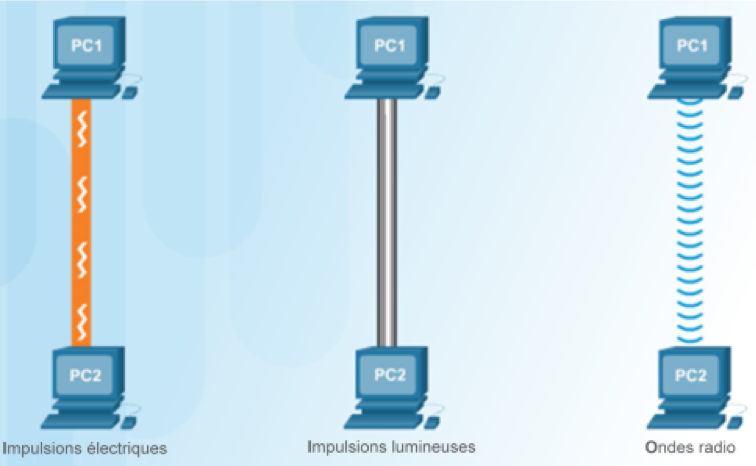
\includegraphics[width=.5\textwidth]{Src/Images/transmission}
  \caption{Transmettre des données}
  \label{fig:transmission}
\end{figure}

Les bits sont transmis sous forme de signaux, à l'aide de câbles de cuivre (impulsions électriques), de câble à fibre optique (impulsions lumineuses) et radio (ondes radio) cd \UPSTIfig{fig:transmission}.

\UPSTIdefinition[Bande passante]{\UPSTIlignesACompleter{La bande passante numérique mesure la quantité d'informations pouvant circuler d'un emplacement à un autre pendant une période donnée. Elle est mesurée en nombre de bits pouvant être transmis (en théorie) pendant une seconde sur un support donné.
}}

\UPSTIdefinition[Débit]{\UPSTIlignesACompleter{Le débit est la mesure du transfert de bits constaté sur le support pendant une période donnée.
}}

\UPSTIaRetenir{En résumé, la bande passante représente le débit maximal.}

\begin{UPSTIactivite}
  \resetNumQuestion
  L'image de la \UPSTIfig{fig:transmission} pèse \SI{119 000}{o}.
  \UPSTIquestion{Combien pèse cette image en \si{Ko} ?}

  \UPSTIlignesACompleter[1]{\SI{119}{Ko}}

  \UPSTIquestion{Un utilisateur télécharge cette image en \SI{500}{ms}. A quel débit moyen l'image a-t-elle été téléchargée ?}

  \UPSTIlignesACompleter{On a téléchargé \SI{119}{Ko} en \SI{500}{ms}. En \SI{1}{s}, on aurait donc pu télécharger $119\times \frac{1}{500e-3} = 119\times 2 = \SI{238}{Ko}.$ Le débit est donc de \SI{238}{Ko/s} }

  Sur un réseau Wifi, la \textbf{bande passante} est de \SI{6}{Mbps} (Megabits par seconde).
  \UPSTIquestion{Convertissez la bande passante en \si{Mo/s} (Mégaoctets par seconde).}

  \UPSTIlignesACompleter[1]{$d = \frac{6}{8} = \SI{750}{ko/s}$}

  \UPSTIquestion{Au minimum, combien faudra-t-il de temps pour transmettre l'image de la \UPSTIfig{fig:transmission} au travers de ce réseau Wifi ?}

  \UPSTIlignesACompleter{La bande passante étant le débit maximal, on fait le calcul avec un débit de \SI{750}{Ko/s}}
\end{UPSTIactivite}


En résumé, sur un réseau, il transite en permanence des données encodés à l'aide de 1 ou de 0 (bits). Ces bits peuvent prendre différentes formes en fonction du signal : lumineux, électriques, ondes-radios, etc.

\section{Clients et serveurs}

Dans un réseau, il cohabite différents types d'hôtes : Les clients et les serveurs.

\UPSTIdefinition[Serveur]{\UPSTIlignesACompleter{Les serveurs sont des hôtes équipés d'un logiciel leur permettant de fournir des informations, comme des e-mails ou des pages Web, à d'autres hôtes sur le réseau.}}

\UPSTIdefinition[Client]{\UPSTIlignesACompleter{Les clients sont des ordinateurs hôtes équipés d'un logiciel qui leur permet de demander des informations auprès du serveur et de les afficher.
}}

\begin{UPSTIactivite}
  \resetNumQuestion
  \UPSTIquestion{A votre avis, quand votre téléphone se connecte à Instagram, est-il un client ou un serveur ?}

  \UPSTIlignesACompleter[1]{C'est un client}

  \UPSTIquestion{A votre avis, quand vous partagez une connexion internet sur votre téléphone, agit-il comme un client ou un serveur ?}

  \UPSTIlignesACompleter[1]{C'est un serveur}

\end{UPSTIactivite}



\end{document}
